\section{Introduction}

Manipulation planning for deformable one-dimensional objects (DOOs) like ropes and cables is challenging due to the high-dimensional state representation of these objects and the cost of simulating their motion. Furthermore, most tasks benefit from multiple arms to control DOO shape and avoid becoming tangled with the environment. Therefore, the planner needs to consider the DOO, the arms manipulating it, and the environment. A task and motion planning (TAMP) approach to this problem would decompose planning into a grasp selection problem and a motion planning problem for the DOO given a specific grasp, as in \cite{RitaCableRouting,Nair2017,CFM}. However, the DOO planning problems are often expensive to solve. To reduce the space of grasps we need to search, we borrow the idea of a \textit{signature} from the field of topology.

\begin{figure}
    \centering
    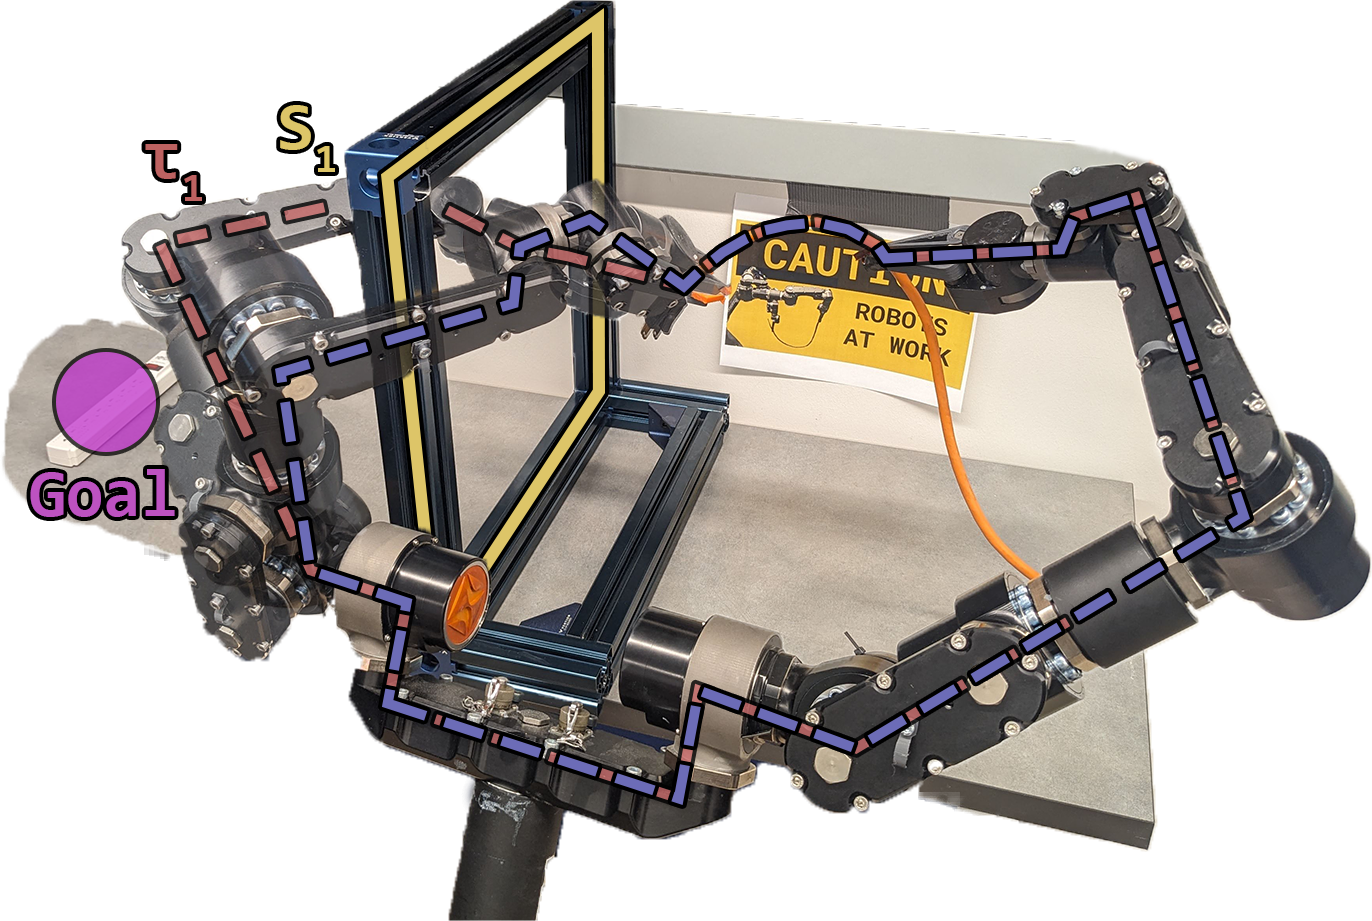
\includegraphics[width=0.8\linewidth]{Chap5/images/real_robot.png}
    \caption{Annotated image of our real world cable threading setup. The red dashed line shows a grasp loop $\tau_1$ that is linked with the skeleton $\skel_1$. The blue grasp loop is not linked with $\skel_1$. This distinction is captured by the proposed \signature{} and is used in planning.}
    \label{fig:titleFig}
\end{figure}

To explain what this signature represents, consider how the robot should grasp the tip of the cable in Figure \ref{fig:titleFig}. By grasping we form a loop, which we call a \textit{grasp loop} and show as blue and red dashed lines in Figure \ref{fig:titleFig}. It is possible to grasp either around the left side or the right side of the frame, but these two grasps are categorically different in that we cannot smoothly deform from one to the other without breaking the grasp or the frame. The frame also forms a loop, called an obstacle loop. When grasping from the left (red), these two loops are linked, but when grasping from the right (blue) they are not. Our key insight is that the robot, DOO, and environment form a \textit{graph of grasp loops} and we can use this graph to construct a signature, \signature{}, which captures topological information relevant for planning. To be clear, we do not address knots in the DOO. Our work is complimentary to work on tying or untying knots \cite{WakamatsuKnots2005, Saha07, UntanglingFull, WeifuKnots}.

The main contribution of this paper is the \signature{} which compactly represents the topology of both the object and the arms manipulating it. We claim this signature is applicable to many systems and is useful for manipulation planning. Figure \ref{fig:examples} shows three examples where we demonstrate planning, and two more examples where the \signature{} may be useful. In simulation, we show that methods using the \signature{} outperform baselines and ablations which search for grasps without using topological information. Finally, we demonstrate a threading and point reaching task on a physical robot. Videos and animations can be found on our Project Website\footnote{\href{https://sites.google.com/view/doo-manipulation-signature/home}{https://sites.google.com/view/doo-manipulation-signature/home}}.

% TODO: rewrite this bit
In the remainder of this paper, we first review related work and then define the \signature{}. Next, we describe a method for DOO manipulation that demonstrates the utility of the \signature{}. Section VI describes how this method can be applied in three environments, which we call Pulling, Untangling, and Threading. We conclude with a brief discussion of our real world demonstration of the Threading task, which is depicted in Figure \ref{fig:titleFig}.
